\chapter{Sel: Satuan Bersama Kehidupan}\label{ch:g10:cells-common-unit}

Keroklah bagian dalam pipimu dengan kapas bertangkai, oleskan pada kaca
objek, tambahkan setetes zat warna biru, lalu tengok lewat mikroskop
pada \omterm{def:g10:cells-common-unit:magnification}{perbesaran} empat ratus kali: sebaran ubin pipih tak beraturan,
masing-masing dengan bintik gelap di dekat pusatnya. Kelupas selaput
tipis dari sisik bawang bombai dan tengok lagi: bata persegi panjang
yang rapi, masing-masing dengan bintiknya sendiri. Air kolam
memperlihatkan makhluk lonjong yang mendayung lewat dengan rumbai bulu.
Ketiga cuplikan itu tidak punya kesamaan bagi mata telanjang. Di bawah
lensa ketiganya dibangun dari benda yang sama --- \omterm{def:g10:cells-common-unit:cell}{sel} --- dan bab ini
membahas benda apa itu, bagaimana ia dilihat, dan mengapa setiap
makhluk hidup terbuat darinya.

\section{Teori sel}

\begin{definition}[Sel]\label{def:g10:cells-common-unit:cell}
Sebuah \emph{sel}\index{sel} adalah satuan terkecil makhluk hidup yang
dirinya sendiri hidup: sebuah volume isi berair, yaitu
\emph{sitoplasma}\index{sitoplasma}, yang terkurung oleh
\emph{membran plasma}\index{membran plasma} tipis yang memisahkannya
dari lingkungannya sambil membiarkan zat terpilih menyeberang. Sebuah
sel menerima materi dan energi, mengubahnya, tumbuh, dan membelah
menjadi dua sel.
\end{definition}

\begin{proposition}[Teori sel]\label{prop:g10:cells-common-unit:theory}
Tiga pernyataan, yang ditegakkan lewat mikroskopi pada abad
kesembilan belas, membentuk teori \omterm{def:g10:cells-common-unit:cell}{sel}:
\begin{enumerate}
  \item setiap makhluk hidup terbuat dari satu \omterm{def:g10:cells-common-unit:cell}{sel} atau lebih;
  \item \omterm{def:g10:cells-common-unit:cell}{sel} adalah satuan dasar struktur dan fungsi makhluk
        hidup --- tidak ada yang lebih kecil yang hidup sendirian;
  \item setiap \omterm{def:g10:cells-common-unit:cell}{sel} berasal dari \omterm{def:g10:cells-common-unit:cell}{sel} yang sudah ada sebelumnya, lewat pembelahan.
\end{enumerate}
\end{proposition}
\begin{proof}[Bukti percobaan]
Pernyataan 1 bersandar pada pemeriksaan sistematis tumbuhan (Schleiden,
1838) dan hewan (Schwann, 1839) dengan mikroskop yang lebih baik:
setiap jaringan yang diperiksa, betapa pun berbeda rupanya, terurai
menjadi \omterm{def:g10:cells-common-unit:cell}{sel}. Pernyataan 3 ditegakkan oleh Virchow (1855) dan oleh
pengamatan \omterm{def:g10:cells-common-unit:cell}{sel} yang membelah dalam jaringan yang sedang tumbuh;
kemungkinan lain --- \omterm{def:g10:cells-common-unit:cell}{sel} yang terbentuk dengan sendirinya dari cairan
--- tidak pernah teramati, dan percobaan Pasteur atas mikroba
(\cref{ch:g11:antibiotic-resistance} kembali kepadanya) menutup
persoalan itu. Pernyataan 2 mengikuti dari yang pertama dan dari
kenyataan bahwa \omterm{def:g10:cells-common-unit:cell}{sel} yang terpencil, jika dipelihara dalam cairan yang
cocok, terus hidup sedangkan serpihan \omterm{def:g10:cells-common-unit:cell}{sel} mana pun tidak.
\end{proof}

\begin{example}[Satu sel atau banyak]\label{ex:g10:cells-common-unit:onemany}
Ragi, paramesium atau bakteri adalah \omterm{def:g10:cells-common-unit:cell}{sel} tunggal yang mengerjakan
segalanya --- makan, bergerak, membelah. Pohon ek atau manusia adalah
kerja sama \omterm{def:g10:cells-common-unit:cell}{sel} dari banyak jenis, masing-masing memikul sebagian
pekerjaan: tubuh manusia memuat sekitar $\num{3e13}$ \omterm{def:g10:cells-common-unit:cell}{sel}, dari kira-kira
dua ratus jenis. Di antara keduanya terletak koloni dan organisme
bersel banyak yang sederhana, tetapi tidak ada makhluk hidup yang
dibangun dari sesuatu selain \omterm{def:g10:cells-common-unit:cell}{sel}.
\end{example}

\section{Melihat sel: skala dan mikroskop}

\begin{definition}[Perbesaran dan daya pisah]\label{def:g10:cells-common-unit:magnification}
Yang disebut \emph{perbesaran}\index{perbesaran} sebuah alat adalah
nisbah ukuran bayangan terhadap ukuran bendanya. Yang disebut
\emph{daya pisah}\index{daya pisah} adalah jarak terkecil antara dua
titik yang masih diperlihatkannya secara terpisah. Memperbesar bayangan
melampaui apa yang dibenarkan daya pisahnya memperbesar kaburnya, bukan
rinciannya.
\end{definition}

\begin{proposition}[Dua alat, dua skala]\label{prop:g10:cells-common-unit:microscopes}
Mikroskop cahaya memperbesar sampai sekitar $\times 1500$ dengan \omterm{def:g10:cells-common-unit:magnification}{daya
pisah} sekitar \qty{0.2}{\micro m}: ia memperlihatkan \omterm{def:g10:cells-common-unit:cell}{sel}, \omterm{def:g10:cells-common-unit:organelle}{inti sel},
\omterm{def:g10:cells-common-unit:organelle}{kloroplas} dan bakteri, berwarna dan hidup. Mikroskop elektron memakai
berkas elektron sebagai ganti cahaya: \omterm{def:g10:cells-common-unit:magnification}{daya pisah} di bawah
\qty{1}{nm}, \omterm{def:g10:cells-common-unit:magnification}{perbesaran} sampai $\times 10^6$; ia menyingkapkan
struktur dalam \omterm{def:g10:cells-common-unit:cell}{sel} --- membran, \omterm{def:g10:cells-common-unit:organelle}{mitokondria}, \omterm{def:g10:cells-common-unit:organelle}{ribosom}, bahkan molekul
besar --- tetapi pada cuplikan yang mati, kering dan diiris menjadi
lapisan yang lebih tipis daripada satu mikrometer.
\end{proposition}
\admitted

\begin{omfigure}
\begin{tikzpicture}[>=Stealth]
  % log scale ruler from 1 nm (0) to 1 m (9 decades), 1.3 cm per decade
  \draw[thick] (0,0) -- (11.7,0);
  \foreach \d/\t in {0/{\qty{1}{nm}}, 1/{\qty{10}{nm}}, 2/{\qty{100}{nm}},
      3/{\qty{1}{\micro m}}, 4/{\qty{10}{\micro m}}, 5/{\qty{100}{\micro m}},
      6/{\qty{1}{mm}}, 7/{\qty{1}{cm}}, 8/{\qty{10}{cm}}, 9/{\qty{1}{m}}}
    \draw (1.3*\d,0.12) -- (1.3*\d,-0.12) node[below, font=\scriptsize] {\t};
  % objects above the ruler
  \foreach \d/\h/\t in {0.3/0.5/{lebar DNA}, 0.9/1.1/{protein},
      2.0/0.5/{virus}, 3.0/1.1/{bakteri}, 4.3/0.5/{sel hewan},
      4.9/1.1/{sel tumbuhan}, 6.0/0.5/{telur katak}, 6.9/1.1/{semut},
      8.3/0.5/{manusia}}
    \node[font=\scriptsize, anchor=south] at (1.3*\d,\h) {\t};
  \foreach \d in {0.3,0.9,2.0,3.0,4.3,4.9,6.0,6.9,8.3}
    \fill (1.3*\d,0) circle (1.6pt);
  \foreach \d/\h in {0.9/1.1,3.0/1.1,4.9/1.1,6.9/1.1}
    \draw[gray] (1.3*\d,0.05) -- (1.3*\d,\h);
  \foreach \d/\h in {0.3/0.5,2.0/0.5,4.3/0.5,6.0/0.5,8.3/0.5}
    \draw[gray] (1.3*\d,0.05) -- (1.3*\d,\h);
  % instrument ranges below
  \draw[<->, omDef, thick] (0,-1.0) -- (3.9,-1.0)
    node[midway, below, font=\scriptsize, omDef] {mikroskop elektron};
  \draw[<->, omProp, thick] (2.6,-1.6) -- (6.5,-1.6)
    node[midway, below, font=\scriptsize, omProp] {mikroskop cahaya};
  \draw[<->, omMeth, thick] (5.9,-2.2) -- (11.7,-2.2)
    node[midway, below, font=\scriptsize, omMeth] {mata telanjang};
\end{tikzpicture}

{\small Ukuran pada skala logaritmik: tiap langkah sepuluh kali lebih
besar. Mata telanjang memisahkan sekitar \qty{0.1}{mm}; mikroskop
cahaya mencapai \qty{0.2}{\micro m} dan melihat \omterm{def:g10:cells-common-unit:cell}{sel} utuh serta bakteri;
mikroskop elektron memisahkan nanometer dan memperlihatkan bagian di dalamnya.}
\end{omfigure}

\begin{method}[Mengukur benda pada sebuah mikrograf]\label{met:g10:cells-common-unit:measure}
Sebuah mikrograf membawa \omterm{def:g10:cells-common-unit:magnification}{perbesaran} atau batang skala.
\begin{enumerate}
  \item Dengan batang skala: ukur batangnya pada halaman (misalnya
        \qty{12}{mm} untuk batang berlabel \qty{10}{\micro m}) dan
        bendanya (\qty{30}{mm}); ukuran sebenarnya adalah $30 \times 10/12 =
        \qty{25}{\micro m}$.
  \item Dengan \omterm{def:g10:cells-common-unit:magnification}{perbesaran}: ukuran sebenarnya $=$ ukuran terukur dibagi
        \omterm{def:g10:cells-common-unit:magnification}{perbesarannya}; \omterm{def:g10:cells-common-unit:cell}{sel} yang tergambar sepanjang \qty{20}{mm} pada
        $\times 400$ berukuran $20/400 = \qty{0.05}{mm} = \qty{50}{\micro m}$.
  \item Selalu sebutkan satuannya, dan lakukan penyetaraan: $\qty{1}{mm} =
        \qty{1000}{\micro m}$, $\qty{1}{\micro m} = \qty{1000}{nm}$.
\end{enumerate}
\end{method}

\begin{example}[Sel pipi]\label{ex:g10:cells-common-unit:cheek}
\omterm{def:g10:cells-common-unit:cell}{Sel} pipi yang tergambar selebar \qty{24}{mm} dari bayangan $\times 400$
berukuran $24/400 = \qty{0.06}{mm} = \qty{60}{\micro m}$ melintang, dan
\omterm{def:g10:cells-common-unit:organelle}{inti selnya}, yang tergambar \qty{3}{mm}, sekitar \qty{8}{\micro m}. \omterm{def:g10:cells-common-unit:cell}{Sel}
darah merah berukuran \qty{7}{\micro m}; bakteri mulut, yang panjangnya
\qty{1}{\micro m}, tampak sebagai titik yang nyaris tak terpisahkan
pada \omterm{def:g10:cells-common-unit:magnification}{perbesaran} yang sama.
\end{example}

\section{Di dalam sel}

\begin{definition}[Organel]\label{def:g10:cells-common-unit:organelle}
Sebuah \emph{organel}\index{organel} adalah struktur di dalam \omterm{def:g10:cells-common-unit:cell}{sel}, yang
terkurung oleh membrannya sendiri, yang menjalankan satu tugas
tertentu. Yang utama adalah:
\begin{itemize}
  \item \emph{inti sel}\index{inti sel}, yang memuat
        kromosom --- DNA pada \cref{ch:g10:universal-dna} --- dan
        mengendalikan kegiatan \omterm{def:g10:cells-common-unit:cell}{selnya};
  \item \emph{mitokondria}\index{mitokondria}, yang panjangnya sekitar
        \qty{1}{\micro m}, tempat molekul organik dibongkar
        dengan oksigen untuk melepaskan energi yang terpakai (respirasi
        seluler, \cref{ch:g10:cell-metabolism});
  \item pada \omterm{def:g10:cells-common-unit:cell}{sel} tumbuhan, \emph{kloroplas}\index{kloroplas},
        yang hijau oleh klorofil, tempat fotosintesis berlangsung, dan
        \emph{vakuola}\index{vakuola} besar berisi air yang menjaga
        \omterm{def:g10:cells-common-unit:cell}{selnya} tetap tegang.
\end{itemize}
Di luar membrannya, \omterm{def:g10:cells-common-unit:cell}{sel} tumbuhan terkotakkan oleh
\emph{dinding sel}\index{dinding sel} selulosa yang kaku; \omterm{def:g10:cells-common-unit:cell}{sel} hewan
tidak punya. \omterm{def:g10:cells-common-unit:cell}{Sitoplasma} setiap \omterm{def:g10:cells-common-unit:cell}{sel} juga memuat jutaan
\emph{ribosom}\index{ribosom}, partikel berukuran sekitar \qty{25}{nm}
yang merakit \omterm{def:g10:chemistry-of-life:families}{protein}, yang hanya terlihat dengan mikroskop elektron.
\end{definition}

\begin{omfigure}
\begin{tikzpicture}[>=Stealth, font=\small, line cap=round, line join=round]
  % ---------- animal cell ----------
  \begin{scope}
    \draw[thick, fill=omDef!6] (0,0) .. controls (1.4,1.9) and (2.9,0.9) .. (2.4,-0.2)
      .. controls (2.1,-1.5) and (0.6,-2.0) .. (-0.6,-1.6)
      .. controls (-2.4,-1.1) and (-2.6,0.6) .. (-1.4,1.3)
      .. controls (-0.9,1.6) and (-0.5,1.4) .. (0,0) -- cycle;
    % nucleus with nucleolus
    \draw[thick, fill=omDef!30] (-0.4,-0.1) circle (0.72);
    \fill[omDef!70] (-0.55,0.05) circle (0.17);
    \node[font=\scriptsize] at (-0.4,-0.33) {inti sel};
    % mitochondria with cristae
    \foreach \x/\y/\r in {1.3/0.4/25, 1.1/-0.9/-35, -1.5/-0.9/60, 0.5/0.9/-10} {
      \begin{scope}[rotate around={\r:(\x,\y)}]
        \draw[fill=omProp!35] (\x,\y) ellipse (0.36 and 0.17);
        \draw[omProp!80!black, thin] (\x-0.2,\y-0.1) -- (\x-0.2,\y+0.1) (\x-0.07,\y-0.12) -- (\x-0.07,\y+0.12) (\x+0.07,\y-0.12) -- (\x+0.07,\y+0.12) (\x+0.2,\y-0.1) -- (\x+0.2,\y+0.1);
      \end{scope}}
    % ribosomes
    \foreach \x/\y in {0.5/-1.2, -1.6/0.5, 0.9/0.0, -1.3/-0.5, 1.9/-0.4, 0.2/1.2, -0.9/0.9, 1.6/1.0, -0.2/-1.3}
      \fill (\x,\y) circle (1.1pt);
    \node[anchor=north, font=\small\bfseries] at (0,-2.1) {sel hewan};
    \draw[->] (2.8,1.5) node[right, font=\scriptsize] {membran plasma} -- (2.35,0.55);
    \draw[->] (2.8,-1.1) node[right, font=\scriptsize] {mitokondria} -- (1.5,-0.95);
    \draw[->] (2.8,0.3) node[right, font=\scriptsize] {sitoplasma} -- (1.85,-0.25);
  \end{scope}
  % ---------- plant cell ----------
  \begin{scope}[xshift=8.3cm]
    % cellulose wall (thick, pale green) and the membrane just inside it
    \draw[line width=4pt, green!35!black!45, fill=omMeth!10, rounded corners=5pt] (-2.4,-1.8) rectangle (2.4,1.8);
    \draw[thick, black!80, rounded corners=4pt] (-2.22,-1.62) rectangle (2.22,1.62);
    % large central vacuole
    \draw[thick, fill=cyan!8, rounded corners=15pt] (-0.95,-1.05) rectangle (1.95,1.15);
    \node[font=\scriptsize] at (0.5,0.1) {vakuola};
    % nucleus pressed against the wall, with nucleolus
    \draw[thick, fill=omDef!30] (-1.5,0.8) circle (0.62);
    \fill[omDef!70] (-1.7,1.05) circle (0.14);
    \node[font=\scriptsize] at (-1.5,0.68) {inti sel};
    % chloroplasts: lens-shaped, with stacked membranes inside
    \foreach \x/\y/\r in {-1.55/-0.55/75, -0.35/-1.33/0, 1.05/-1.33/0, 0.25/1.38/0, 1.55/1.38/0} {
      \begin{scope}[rotate around={\r:(\x,\y)}]
        \draw[fill=green!55!black!45] (\x,\y) ellipse (0.36 and 0.18);
        \draw[green!25!black, line width=0.9pt] (\x-0.2,\y-0.06) -- (\x-0.2,\y+0.06) (\x-0.08,\y-0.09) -- (\x-0.08,\y+0.09) (\x+0.06,\y-0.09) -- (\x+0.06,\y+0.09) (\x+0.19,\y-0.06) -- (\x+0.19,\y+0.06);
      \end{scope}}
    % mitochondria
    \foreach \x/\y/\r in {-1.75/-1.2/35, -0.75/1.38/0} {
      \begin{scope}[rotate around={\r:(\x,\y)}]
        \draw[fill=omProp!35] (\x,\y) ellipse (0.3 and 0.14);
        \draw[omProp!80!black, thin] (\x-0.14,\y-0.08) -- (\x-0.14,\y+0.08) (\x,\y-0.1) -- (\x,\y+0.1) (\x+0.14,\y-0.08) -- (\x+0.14,\y+0.08);
      \end{scope}}
    % ribosomes in the thin cytoplasm
    \foreach \x/\y in {-1.1/-1.4, 2.08/0.3, 2.08/-0.8, -2.05/0.1, 0.8/1.42, -2.05/-0.9}
      \fill (\x,\y) circle (1.1pt);
    \node[anchor=north, font=\small\bfseries] at (0,-2.1) {sel tumbuhan};
    \draw[->] (2.8,1.7) node[right, font=\scriptsize] {dinding sel} -- (2.45,1.4);
    \draw[->] (2.8,0.9) node[right, font=\scriptsize] {membran plasma} -- (2.24,0.7);
    \draw[->] (2.8,-0.3) node[right, font=\scriptsize] {sitoplasma} -- (2.1,-0.55);
    \draw[->] (2.8,-1.3) node[right, font=\scriptsize] {kloroplas} -- (1.42,-1.33);
  \end{scope}
\end{tikzpicture}

{\small Dua \omterm{def:g10:cells-common-unit:prokaryote}{sel eukariotik}, secara skematis. Keduanya punya membran,
\omterm{def:g10:cells-common-unit:cell}{sitoplasma} dengan \omterm{def:g10:cells-common-unit:organelle}{mitokondria} (jingga) dan \omterm{def:g10:cells-common-unit:organelle}{inti sel}; \omterm{def:g10:cells-common-unit:cell}{sel} tumbuhan
menambahkan dinding selulosa, \omterm{def:g10:cells-common-unit:organelle}{kloroplas} (hijau) dan \omterm{def:g10:cells-common-unit:organelle}{vakuola} pusat yang
besar. Keduanya tidak tergambar sebanding: \omterm{def:g10:cells-common-unit:organelle}{inti sel} sesungguhnya
sekitar sepersepuluh lebar \omterm{def:g10:cells-common-unit:cell}{selnya}, dan \omterm{def:g10:cells-common-unit:organelle}{mitokondria} seratus kali lebih kecil daripada \omterm{def:g10:cells-common-unit:cell}{selnya}.}
\end{omfigure}

\begin{definition}[Prokariot dan eukariot]\label{def:g10:cells-common-unit:prokaryote}
\omterm{def:g10:cells-common-unit:cell}{Sel} yang DNA-nya terkurung dalam \omterm{def:g10:cells-common-unit:organelle}{inti sel} adalah
\emph{sel eukariotik}\index{sel eukariotik}: hewan, tumbuhan, jamur
dan banyak organisme bersel satu tergolong eukariot. Sebuah
\emph{sel prokariotik}\index{sel prokariotik} tidak punya \omterm{def:g10:cells-common-unit:organelle}{inti sel} dan
tidak punya \omterm{def:g10:cells-common-unit:organelle}{organel} bermembran: DNA-nya terletak bebas dalam
\omterm{def:g10:cells-common-unit:cell}{sitoplasma}, ukurannya sekitar \qty{1}{\micro m}, dan ia diselubungi
dinding dari jenisnya sendiri. Bakteri tergolong prokariot.
\end{definition}

\begin{example}[Membaca sebuah bakteri]\label{ex:g10:cells-common-unit:bacterium}
Mikrograf elektron bakteri usus \emph{Escherichia coli}
memperlihatkan batang sepanjang \qty{2}{\micro m} dan selebar
\qty{0.5}{\micro m}: sebuah dinding, membran tepat di dalamnya,
\omterm{def:g10:cells-common-unit:cell}{sitoplasma} berbutir yang padat dengan \omterm{def:g10:cells-common-unit:organelle}{ribosom}, dan daerah tengah yang
lebih pucat tempat satu-satunya molekul DNA melingkar terletak. Tanpa
\omterm{def:g10:cells-common-unit:organelle}{inti sel}, tanpa \omterm{def:g10:cells-common-unit:organelle}{mitokondria}. Namun \omterm{def:g10:cells-common-unit:cell}{selnya} makan, tumbuh dan membelah
tiap dua puluh menit dalam kaldu yang kaya: segala yang dituntut teori
\omterm{def:g10:cells-common-unit:cell}{sel}, dalam seperseribu volume \omterm{def:g10:cells-common-unit:cell}{sel} pipi.
\end{example}

\begin{omfigure}
\begin{tikzpicture}
  \node[anchor=south west, inner sep=0] (img) at (0,0)
    {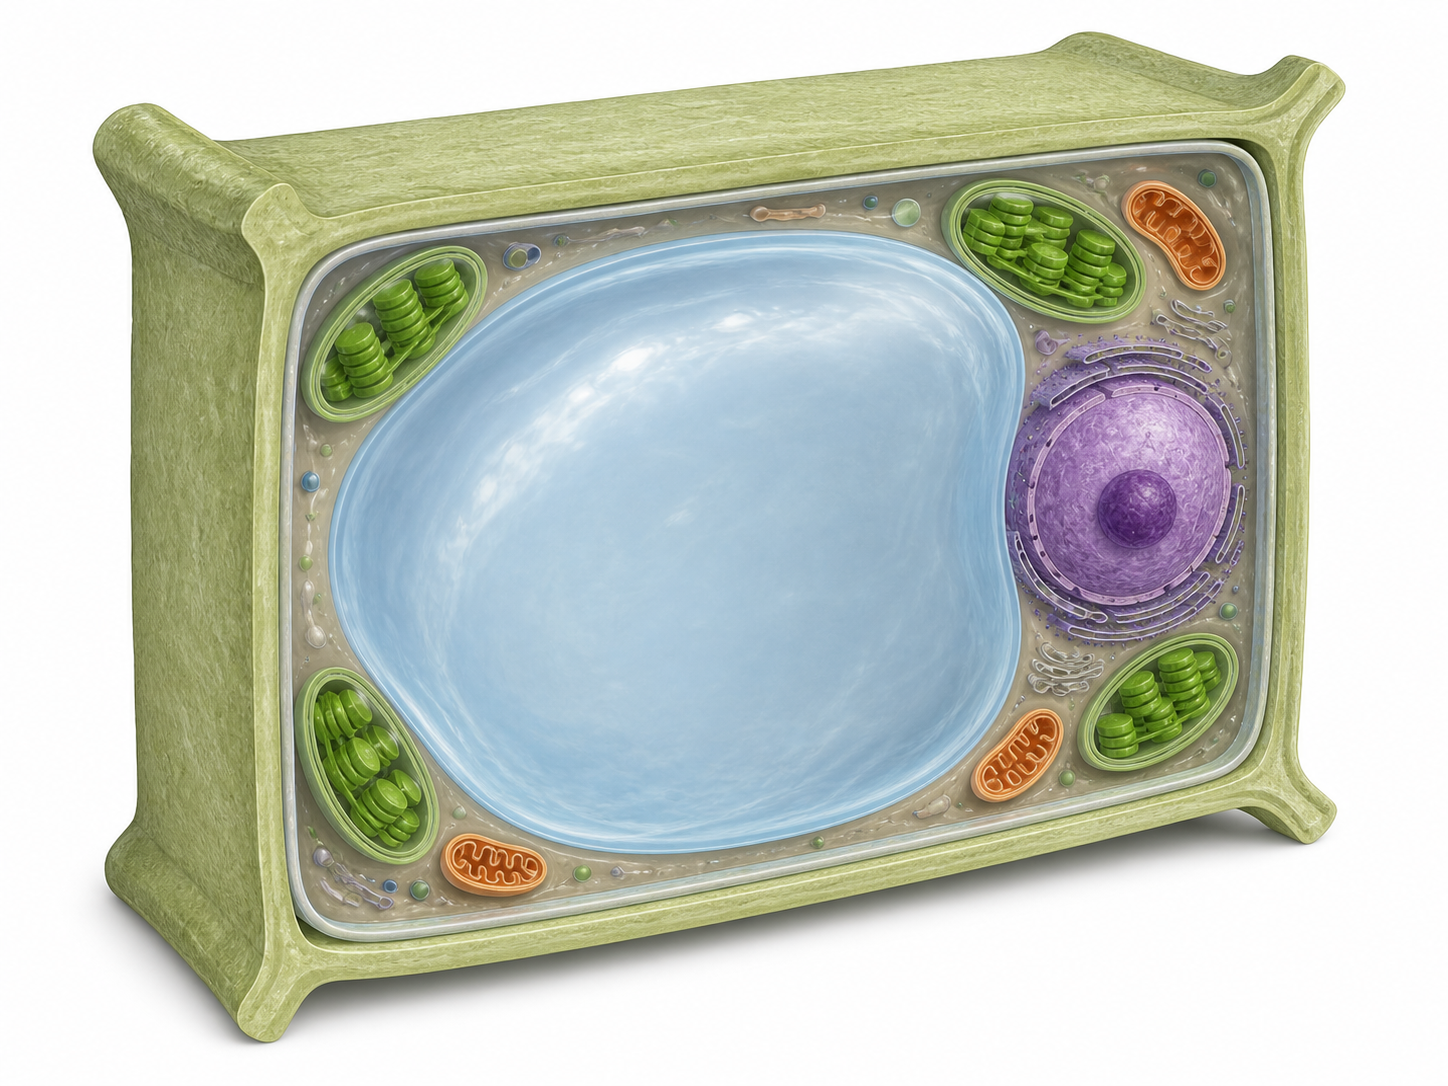
\includegraphics[width=0.52\linewidth]{images/book2/ai/fig-plant-cell-cutaway-v2.png}};
  \begin{scope}[x={(img.south east)}, y={(img.north west)},
      every node/.style={font=\small}]
    \draw[omDef, thick] (0.78,0.54) -- (1.05,0.62) node[right] {inti sel};
    \draw[omDef, thick] (0.92,0.28) -- (1.05,0.18) node[right] {dinding sel};
    \draw[omDef, thick] (0.45,0.54) -- (0.45,1.06) node[above] {vakuola};
    \draw[omDef, thick] (0.215,0.50) -- (-0.05,0.64) node[left] {membran plasma};
    \draw[omDef, thick] (0.25,0.30) -- (-0.05,0.30) node[left] {kloroplas};
    \draw[omDef, thick] (0.34,0.21) -- (-0.05,0.08) node[left] {mitokondria};
  \end{scope}
\end{tikzpicture}

{\small \omterm{def:g10:cells-common-unit:cell}{Sel} tumbuhan yang dibelah: dinding yang kaku, membran tipis
yang menempel padanya, \omterm{def:g10:cells-common-unit:organelle}{inti sel}, \omterm{def:g10:cells-common-unit:organelle}{kloroplas} yang hijau dan \omterm{def:g10:cells-common-unit:organelle}{vakuola} yang
mengisi sebagian besar volumenya.}
\end{omfigure}

\section{Banyak sel, banyak bentuk: spesialisasi}

\begin{proposition}[Sel yang terspesialisasi]\label{prop:g10:cells-common-unit:specialised}
Dalam organisme bersel banyak, \omterm{def:g10:cells-common-unit:cell}{selnya} berbagi rancangan dasar yang sama
dan DNA yang sama, tetapi tiap jenis punya bentuk dan perlengkapan yang
serasi dengan tugasnya: neuron menjulurkan serabut sepanjang satu meter
untuk membawa isyarat; \omterm{def:g10:cells-common-unit:cell}{sel} darah merah telah kehilangan \omterm{def:g10:cells-common-unit:organelle}{inti selnya} dan
berupa cakram pipih yang padat dengan hemoglobin; serat otot adalah \omterm{def:g10:cells-common-unit:cell}{sel}
raksasa yang penuh \omterm{def:g10:chemistry-of-life:families}{protein} yang dapat berkerut; bulu akar berupa tabung
tipis yang memperbesar permukaan untuk menyerap air; \omterm{def:g10:cells-common-unit:cell}{sel} penjaga pada
daun berubah bentuk untuk membuka atau menutup sebuah liang.
Spesialisasi adalah soal bagian mana dari rancangan bersama itu yang dikembangkan.
\end{proposition}
\admitted

\begin{example}[Permukaan dan volume]\label{ex:g10:cells-common-unit:surface}
Mengapa \omterm{def:g10:cells-common-unit:cell}{sel} begitu kecil? Segala yang diterima atau dikeluarkan sebuah
\omterm{def:g10:cells-common-unit:cell}{sel} menyeberangi membrannya, yang luasnya tumbuh menurut kuadrat
ukurannya, sedangkan kebutuhannya tumbuh menurut volumenya, yaitu
pangkat tiga. \omterm{def:g10:cells-common-unit:cell}{Sel} berbentuk kubus bersisi \qty{10}{\micro m} punya
permukaan \qty{600}{\micro m^2} untuk volume \qty{1000}{\micro m^3}:
\qty{0.6}{\micro m^2} membran tiap mikrometer kubik. Pada sisi
\qty{100}{\micro m} nisbahnya turun menjadi \qty{0.06}{\micro m^2}:
sepuluh kali lebih sedikit membran tiap satuan isi. \omterm{def:g10:cells-common-unit:cell}{Sel} yang besar akan
kelaparan di pusatnya; \omterm{def:g10:cells-common-unit:cell}{sel} yang memang besar (telur katak, serat otot)
sebagian besar berupa cadangan yang tidak aktif atau memanjang sehingga
tidak ada titik yang jauh dari permukaannya.
\end{example}

\begin{omfigure}
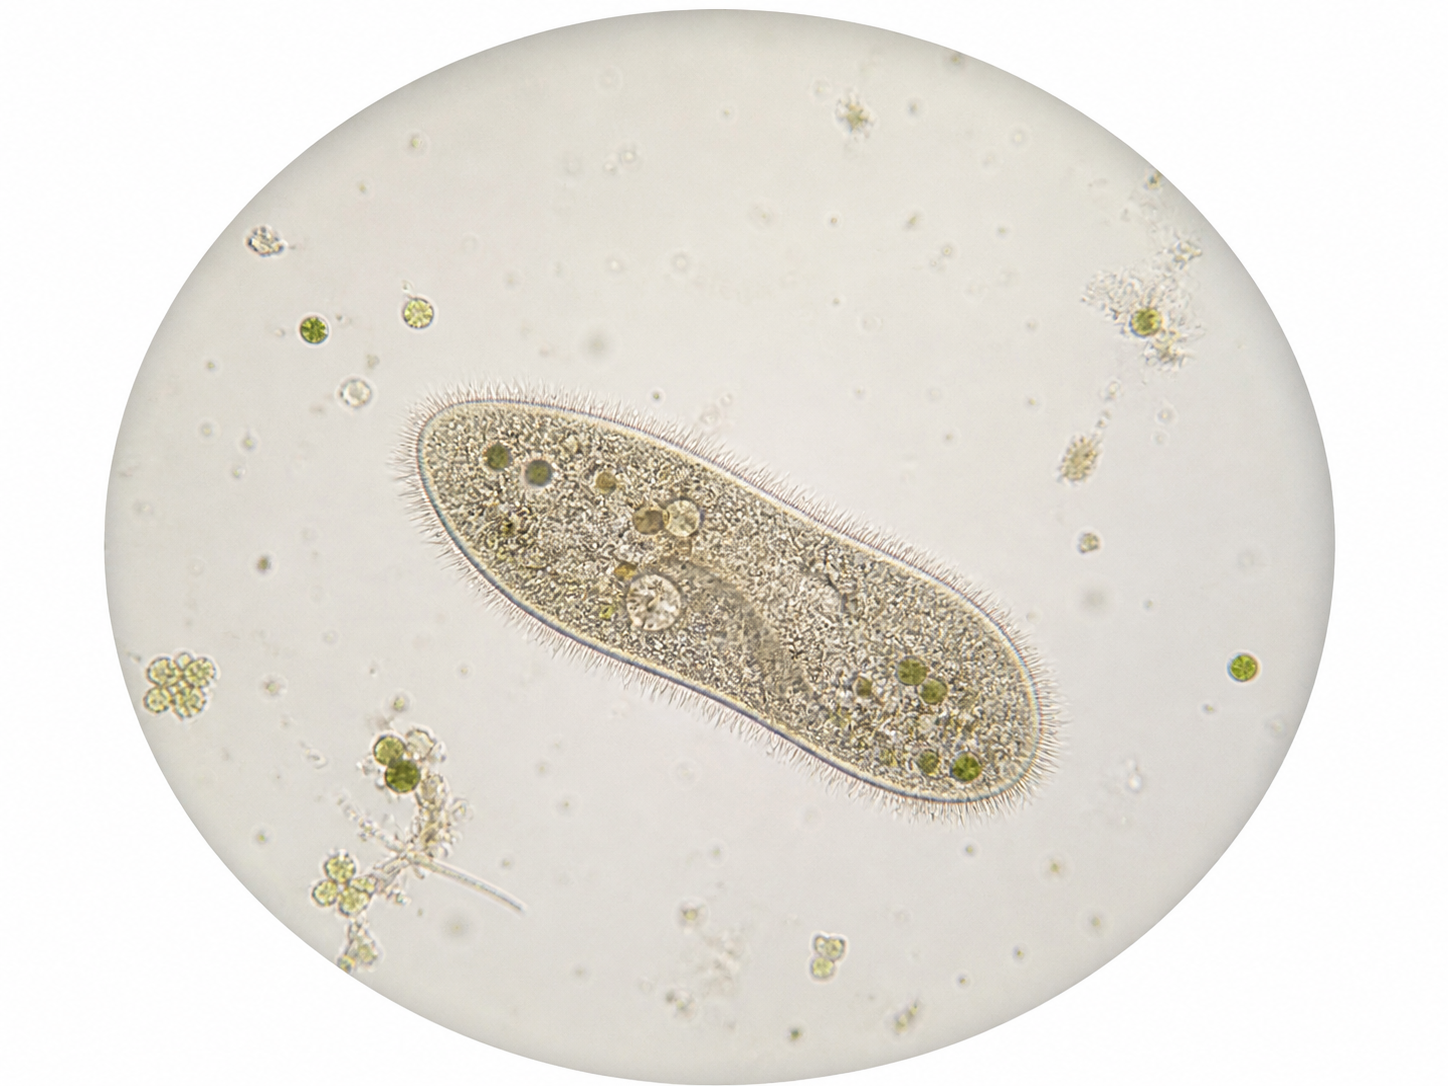
\includegraphics[width=0.62\linewidth]{images/book2/ai/g10-cells-paramecium.png}

{\small Setetes air kolam di bawah mikroskop cahaya: seekor paramesium,
satu \omterm{def:g10:cells-common-unit:cell}{sel} sepanjang seperempat milimeter, mendayung lewat di antara alga
hijau dengan kibasan ribuan bulu halus. Satu \omterm{def:g10:cells-common-unit:cell}{sel}, dan satu organisme utuh.}
\end{omfigure}

\begin{remark}[Sel sebagai sistem terbuka]\label{rem:g10:cells-common-unit:open}
\omterm{def:g10:cells-common-unit:cell}{Sel} bukanlah kantong yang tersegel. Air, oksigen, glukosa dan ion
terus-menerus menyeberangi membrannya, dan sisanya keluar lewat jalan
yang sama; \omterm{def:g10:cells-common-unit:cell}{sel} pipi yang ditaruh dalam air murni menggembung dan pecah
dalam hitungan menit, dan yang ditaruh dalam air asin pekat mengerut.
Kendali membran atas apa yang masuk dan keluar menjadi pokok jilid
Tahun ke-1; untuk sekarang, ingatlah bahwa \omterm{def:g10:cells-common-unit:cell}{sel} hidup dengan bertukar
dengan lingkungannya, dan mati ketika pertukarannya berhenti.
\end{remark}

\section{Latihan}

\begin{exercise}[$\star$]\label{exo:g10:cells-common-unit:1}
Nyatakan ketiga pernyataan teori \omterm{def:g10:cells-common-unit:cell}{sel}.
\end{exercise}

\begin{exercise}[$\star$]\label{exo:g10:cells-common-unit:2}
Setarakan: \qty{0.05}{mm} ke mikrometer; \qty{2500}{nm} ke mikrometer;
\qty{7}{\micro m} ke milimeter.
\end{exercise}

\begin{exercise}[$\star$]\label{exo:g10:cells-common-unit:3}
Sebuah \omterm{def:g10:cells-common-unit:cell}{sel} tergambar sepanjang \qty{36}{mm} dari bayangan $\times 600$.
Berapa panjang sebenarnya?
\end{exercise}

\begin{exercise}[$\star$]\label{exo:g10:cells-common-unit:4}
Sebutkan tiga struktur yang ada pada \omterm{def:g10:cells-common-unit:cell}{sel} tumbuhan tetapi tidak pada \omterm{def:g10:cells-common-unit:cell}{sel}
hewan, dan satu struktur yang ada pada setiap \omterm{def:g10:cells-common-unit:cell}{sel}.
\end{exercise}

\begin{exercise}[$\star$]\label{exo:g10:cells-common-unit:5}
Apa beda \omterm{def:g10:cells-common-unit:prokaryote}{sel prokariotik} dan \omterm{def:g10:cells-common-unit:prokaryote}{sel eukariotik}? Berikan satu contoh
masing-masing.
\end{exercise}

\begin{exercise}[$\star\star$]\label{exo:g10:cells-common-unit:6}
Pada sebuah mikrograf, batang skala berlabel \qty{5}{\micro m} terukur
\qty{15}{mm}; satu \omterm{def:g10:cells-common-unit:organelle}{mitokondria} terukur sepanjang \qty{6}{mm}. Hitung
panjang \omterm{def:g10:cells-common-unit:organelle}{mitokondria} sebenarnya dan \omterm{def:g10:cells-common-unit:magnification}{perbesaran} bayangannya.
\end{exercise}

\begin{exercise}[$\star\star$]\label{exo:g10:cells-common-unit:7}
Mengapa mikroskop cahaya tidak dapat memperlihatkan \omterm{def:g10:cells-common-unit:organelle}{ribosom}, berapa pun
\omterm{def:g10:cells-common-unit:magnification}{perbesarannya}? Pakai kedua istilah pada
\cref{def:g10:cells-common-unit:magnification}.
\end{exercise}

\begin{exercise}[$\star\star$]\label{exo:g10:cells-common-unit:8}
Larutan iodin diteteskan pada sepotong kentang di bawah mikroskop:
warna biru kehitaman muncul dalam butiran lonjong di dalam \omterm{def:g10:cells-common-unit:cell}{selnya}.
Dengan \cref{ch:g10:chemistry-of-life}, sebutkan butiran itu apa dan
apa yang ditunjukkannya tentang tempat tumbuhan menyimpan cadangannya.
\end{exercise}

\begin{exercise}[$\star\star$]\label{exo:g10:cells-common-unit:9}
\omterm{def:g10:cells-common-unit:cell}{Sel} selaput bawang bombai memperlihatkan \omterm{def:g10:cells-common-unit:organelle}{inti sel} dan dinding tetapi
tanpa \omterm{def:g10:cells-common-unit:organelle}{kloroplas}, sedangkan \omterm{def:g10:cells-common-unit:cell}{sel} daun lumut penuh dengannya. Jelaskan
bedanya dari tempat tinggal masing-masing jaringan.
\end{exercise}

\begin{exercise}[$\star\star$]\label{exo:g10:cells-common-unit:10}
Hitung nisbah permukaan terhadap volume \omterm{def:g10:cells-common-unit:cell}{sel} berbentuk kubus bersisi
\qty{1}{\micro m} (sebuah bakteri) dan bersisi \qty{20}{\micro m}
(\omterm{def:g10:cells-common-unit:cell}{sel} hewan yang lazim). Mana yang dapat bersandar pada
peresapan sederhana lewat membrannya saja?
\end{exercise}

\begin{exercise}[$\star\star$]\label{exo:g10:cells-common-unit:11}
Sebuah bakteri dalam kaldu yang kaya membelah tiap \qty{20}{min}. Mulai
dari satu \omterm{def:g10:cells-common-unit:cell}{sel}, ada berapa \omterm{def:g10:cells-common-unit:cell}{sel} setelah \qty{2}{h}? Setelah \qty{4}{h}?
\end{exercise}

\begin{exercise}[$\star\star\star$]\label{exo:g10:cells-common-unit:12}
\omterm{def:g10:cells-common-unit:cell}{Sel} darah merah tidak punya \omterm{def:g10:cells-common-unit:organelle}{inti sel} dan tidak punya \omterm{def:g10:cells-common-unit:organelle}{mitokondria}.
Apakah ia memenuhi \cref{def:g10:cells-common-unit:cell}? Bahaslah,
dengan mengetahui bahwa ia hidup sekitar 120 hari, tidak dapat
membelah, dan dihasilkan oleh \omterm{def:g10:cells-common-unit:cell}{sel} berinti di dalam sumsum tulang.
\end{exercise}

\begin{exercise}[$\star\star\star$]\label{exo:g10:cells-common-unit:13}
Pada 1665 Hooke melihat ``\omterm{def:g10:cells-common-unit:cell}{sel}'' dalam irisan gabus --- kotak kosong
berdinding tebal. Jelaskan apa yang sesungguhnya dilihatnya, dalam
istilah bab ini, dan mengapa ia tidak mungkin melihat \omterm{def:g10:cells-common-unit:organelle}{inti sel} di sana.
\end{exercise}

\begin{exercise}[$\star\star\star$]\label{exo:g10:cells-common-unit:14}
Virus berupa partikel berukuran \qty{20}{nm} sampai \qty{300}{nm} yang
memuat \omterm{def:g10:chemistry-of-life:families}{asam nukleat} dan \omterm{def:g10:chemistry-of-life:families}{protein}, tidak dapat tumbuh atau membelah
sendiri, dan hanya berlipat ganda di dalam \omterm{def:g10:cells-common-unit:cell}{sel}. Apakah virus itu \omterm{def:g10:cells-common-unit:cell}{sel}?
Apakah virus hidup? Berdebatlah dari teori \omterm{def:g10:cells-common-unit:cell}{sel}.
\end{exercise}

\begin{exercise}[$\star\star\star$]\label{exo:g10:cells-common-unit:15}
Serat otot adalah \omterm{def:g10:cells-common-unit:cell}{sel} tunggal sepanjang \qty{3}{cm} dan selebar
\qty{50}{\micro m}, yang memuat ratusan \omterm{def:g10:cells-common-unit:organelle}{inti sel}. Hitung volumenya dan
bandingkan dengan volume \omterm{def:g10:cells-common-unit:cell}{sel} kubus \qty{20}{\micro m}; lalu jelaskan,
dari \cref{ex:g10:cells-common-unit:surface}, mengapa bentuknya dan
banyaknya \omterm{def:g10:cells-common-unit:organelle}{inti sel} membuat ukuran sebesar itu dapat bekerja.
\end{exercise}

\section{Soal: Menghitung Sel dalam Sebuah Tubuh}

\begin{problem}[{Soal akhir pekan --- satu sesi mikroskop, dari selaput
bawang bombai di kaca objek sampai taksiran jumlah sel dalam tubuh
manusia}]
\label{pb:g10:cells-common-unit:1}
Sebuah kelas menghabiskan satu siang di depan mikroskop. Lensa objektif
yang tersedia memberi \omterm{def:g10:cells-common-unit:magnification}{perbesaran} total $\times 40$, $\times 100$ dan
$\times 400$; bidang pandang pada $\times 100$ selebar \qty{1.8}{mm}.

\medskip
\noindent\textbf{Bagian I --- Bawang bombainya.}
\begin{enumerate}
  \item Pada $\times 100$, sekitar 9 \omterm{def:g10:cells-common-unit:cell}{sel} bawang bombai muat
        berdampingan melintasi bidang pandang. Perkirakan lebar satu
        \omterm{def:g10:cells-common-unit:cell}{sel}, dalam mikrometer.
  \item Pada $\times 400$ bidang pandangnya empat kali lebih sempit.
        Berapa lebarnya, dan berapa banyak \omterm{def:g10:cells-common-unit:cell}{sel} itu yang muat melintasinya?
  \item Seorang murid menggambar satu \omterm{def:g10:cells-common-unit:cell}{sel} selebar \qty{28}{mm} dari
        bayangan $\times 400$. Berapa \omterm{def:g10:cells-common-unit:magnification}{perbesaran} gambar itu terhadap
        \omterm{def:g10:cells-common-unit:cell}{sel} yang sebenarnya?
  \item Iodin mewarnai \omterm{def:g10:cells-common-unit:organelle}{inti selnya} cokelat kekuningan; murid itu
        mengukurnya \qty{4}{mm} pada gambarnya. Berapa garis tengah sebenarnya?
  \item Sebutkan struktur yang harus dilabeli murid itu pada gambarnya,
        dan satu struktur yang hadir tetapi tidak dapat terlihat pada
        \omterm{def:g10:cells-common-unit:magnification}{perbesaran} ini.
\end{enumerate}

\medskip
\noindent\textbf{Bagian II --- Pipi dan kolamnya.}
\begin{enumerate}[resume]
  \item \omterm{def:g10:cells-common-unit:cell}{Sel} pipi yang diwarnai biru metilena tampak sebagai poligon
        pipih selebar sekitar \qty{60}{\micro m} tetapi setebal
        \qty{5}{\micro m} saja. Mengapa \omterm{def:g10:cells-common-unit:cell}{sel} itu pipih, mengingat dari
        mana asalnya?
  \item Setetes air kolam memperlihatkan paramesium sepanjang
        \qty{240}{\micro m}. Dapatkah ia terlihat dengan mata
        telanjang? Pada \omterm{def:g10:cells-common-unit:magnification}{perbesaran} mana ia mengisi seperempat bidang pandang?
  \item Titik bergerak yang mungil, panjangnya sekitar
        \qty{1}{\micro m}, terlihat di dekat paramesium itu pada
        $\times 400$. Kemungkinan besar itu apa, dan apa yang akan
        ditambahkan mikroskop elektron?
  \item Paramesium adalah \omterm{def:g10:cells-common-unit:cell}{sel} tunggal; \omterm{def:g10:cells-common-unit:cell}{sel} pipi adalah satu dari
        triliunan. Dalam satu kalimat untuk masing-masing, sebutkan apa
        arti ``terspesialisasi'' bagi \omterm{def:g10:cells-common-unit:cell}{sel} pipi dan mengapa itu tidak
        dapat berlaku bagi paramesium.
  \item Seorang murid meneteskan air asin pada \omterm{def:g10:cells-common-unit:cell}{sel} pipinya dan melihat
        \omterm{def:g10:cells-common-unit:cell}{sel} itu mengerut. Jelaskan dengan
        \cref{rem:g10:cells-common-unit:open}.
\end{enumerate}

\medskip
\noindent\textbf{Bagian III --- Ukuran sebuah \omterm{def:g10:cells-common-unit:cell}{sel}.}
\begin{enumerate}[resume]
  \item Ambil \omterm{def:g10:cells-common-unit:cell}{sel} manusia yang lazim sebagai kubus bersisi \qty{20}{\micro m}.
        Hitung volumenya dalam mikrometer kubik, lalu dalam milimeter
        kubik ($\qty{1}{mm^3} = 10^9\,\unit{\micro m^3}$).
  \item Hitung luas permukaannya dan nisbah permukaan terhadap volume.
  \item Ulangi untuk bakteri yang diambil sebagai kubus bersisi
        \qty{1}{\micro m}. Berapa kali lipat nisbahnya lebih besar?
  \item \omterm{def:g10:cells-common-unit:cell}{Sel} menempati massa yang kira-kira sama dengan massa air yang
        volumenya sama ($\qty{1}{g}$ tiap \unit{cm^3}). Perkirakan massa
        \omterm{def:g10:cells-common-unit:cell}{sel} \qty{20}{\micro m} itu dalam nanogram
        ($\qty{1}{g} = 10^9\,\unit{ng}$).
  \item \omterm{def:g10:cells-common-unit:cell}{Sel} darah merah berupa cakram selebar \qty{7}{\micro m} dan
        setebal \qty{2}{\micro m}. Perkirakan volumenya (perlakukan
        sebagai tabung, $V = \pi r^2 h$) dan bandingkan dengan kubus
        pada pertanyaan 11.
\end{enumerate}

\medskip
\noindent\textbf{Bagian IV --- Jumlah \omterm{def:g10:cells-common-unit:cell}{sel} dalam sebuah tubuh.}
\begin{enumerate}[resume]
  \item Seorang murid bermassa \qty{60}{kg} punya volume sekitar
        \qty{60}{L}. Jika tubuhnya hanya terbuat dari \omterm{def:g10:cells-common-unit:cell}{sel} kubus
        \qty{20}{\micro m}, berapa banyak \omterm{def:g10:cells-common-unit:cell}{sel} yang dimuatnya?
  \item Sesungguhnya sekitar sepertiga volume tubuh berupa cairan di
        antara \omterm{def:g10:cells-common-unit:cell}{selnya} dan bahan bukan \omterm{def:g10:cells-common-unit:cell}{sel} lainnya. Perbaiki taksiran itu.
  \item \omterm{def:g10:cells-common-unit:cell}{Sel} darah merah saja berjumlah sekitar $\num{2.5e13}$. Dengan
        volume pada pertanyaan 15, berapa volume yang ditempatinya?
        Apakah itu sesuai dengan volume darah sekitar \qty{4.5}{L} yang
        45\% di antaranya berupa \omterm{def:g10:cells-common-unit:cell}{sel}?
  \item Gabungkan pertanyaan 17 dan 18: berikan orde besar jumlah
        seluruh \omterm{def:g10:cells-common-unit:cell}{sel} dalam tubuh, dan sebutkan mengapa penghitungan yang
        cermat tidak mungkin.
  \item Nyatakan hasilnya: kira-kira berapa banyak \omterm{def:g10:cells-common-unit:cell}{sel} yang menyusun
        seorang manusia, dan lewat proses apa --- dari berapa jumlah
        awal --- semuanya dihasilkan?
\end{enumerate}
\end{problem}
